\subsection{Incenter Locus Recap}

Consider an Elliptic Billiard \cite{sergei91} centered at $O$, and an $N=3$ periodic trajectory $P_1P_2P_3$, called an {\em orbit}, shown in Figure~\ref{fig:single-orbit}. A vertex bisector is congruent with inward normal to the Ellipse, and these meet at the Incenter $X_1$ \cite{etc}.\\

\noindent Note: Triangular centers (such as the Incenter, Barycenter, etc.) will be referred here by their Kimberling Codes \cite{etc}: $X_1$ for the Incenter, $X_2$ for the Barycenter, etc. Also, $a$ refers to the the Billiard's axis ratio and when not specified, $a=1.5$.

\begin{figure}[H]
     \centering
     \begin{subfigure}[t]{0.45\textwidth}
         \centering
         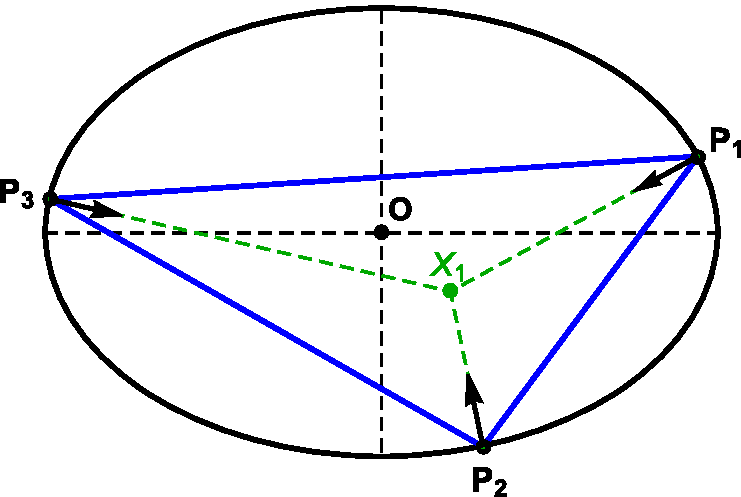
\includegraphics[height=.65 \linewidth]{pics/0000_single_orbit.pdf}
         \caption{An $N=3$ periodic trajectory, called an {\em orbit}, and its Incenter $X_1$: where the bisectors concur.}
         \label{fig:single-orbit}
     \end{subfigure}
     \hfill
     \begin{subfigure}[t]{0.45\textwidth}
         \centering
          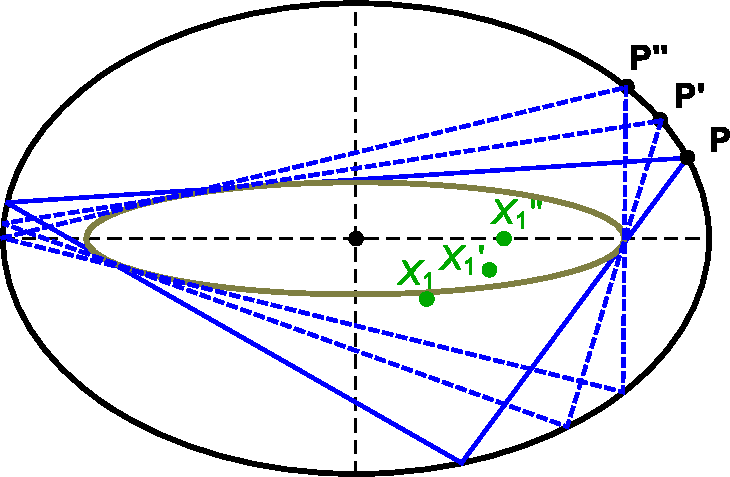
\includegraphics[height=.65\linewidth]{pics/0010_three_orbits.pdf}
         \caption{Three triangular orbits, each associated with a {\em leader} vertex $P,P',P''$, and their Incenters $X_1,X_1',X_1''$, and the confocal Caustic.}
         \label{fig:three-orbits}
     \end{subfigure}
     \caption{Triangular Orbits in an Elliptic Billiard and their Incenter.}
\end{figure}

Poncelet's Porism \cite{dragovic11} states that if one $N$-periodic trajectory can be found starting at a point $P$ on the boundary, then every boundary point can also initiate an $N$-trajectory, i.e., there exists a one-dimensional {\em family} of orbits.

The ellipse is the only planar Billiard with an Integrable Hamiltonian \cite{birkhoff66}. A well-known corollary is that all orbits will have fixed perimeter $L$. For $N=3$ we have derived its expression with respect to the Billiard's aspect ratio: \cite{ronaldo19a}:

\begin{eqnarray}
L&=&\frac{2(\delta+a^2+1)\sqrt{2\delta-a^2-1}}{a^2-1}\\
\delta&=&\sqrt{a^4-a^2+1}
\end{eqnarray}

Joachimsthal's Integral  \cite{sergei91} states that a positive quantity $\gamma$, called the {\em angular momentum} is conserved. This is the scalar product of velocity with the gradient at any orbit vertex:

\begin{equation}
 \gamma=\hat{v}.\nabla{f}(P)=\mbox{constant},\forall{P}
 \label{eqn:joachim}
\end{equation}

\noindent where $P$ is a vertex of the orbit, $\hat{v}$ is the incoming orbit edge, and:

\begin{equation}
f=\frac{1}{2}\left(\frac{x^2}{a^2}+\frac{y^2}{b^2}\right)
\label{eqn:f}
\end{equation}

Geometrically, constant $\gamma$ is equivalent to stating all trajectory edges are tangent to a confocal ellipse, called the {\em Caustic}, Figure~\ref{fig:three-orbits}. For $N=3$ we can express it in terms of the Billiard aspect ratio:

\begin{equation}
\gamma = \frac{\sqrt{2\delta-a^2-1}}{a^2-1}
\label{eqn:gamma}
\end{equation}


Consider the three $N=3$ orbits in Figure~\ref{fig:three-orbits}, identified by a starting vertex $P,P',P''$, called the {\em leader}, as well as their Incenters $X_1,X_1',X_1''$. Let the leader be parametrized continuously:

\begin{equation}
P_1(t)=\left(a\cos{t},\sin{t}\right),\,t\in\left[0,2\pi\right)
\label{eqn:tparam}
\end{equation}

In \cite{ronaldo19} we are provided explicit equations for $P_2$ and $P_3$ in terms of $P_1$, and the dependence is highly non-linear. Though the Incenter's trilinear coordinates \cite{mw} are of the simplest form, $1:1:1$ \cite{etc}, its Cartesian location will be non-trivial given $P_2,P_3$ non-linearities. This renders remarkable the following theorem, which we borrow from \cite{olga14}: 

\begin{theorem}
The locus of the Incenter is elliptic.
\end{theorem}

Also elliptic are the loci of the Barycenter $X_2$, the Circumcenter $X_3$, the Orthocenter $X_4$, and the 9-Point Circle Center $X_5$ \cite{sergei2016,corentin19,ronaldo19}, Figure~\ref{fig:locus-x12345}. These can be viewed as an animation \cite[video \#1]{dsr_main_videos_2019} and interactively \cite{dsr_applet_x12345}.

\begin{figure}[H]
     \centering
     \begin{subfigure}[m]{0.45\textwidth}
     \centering
     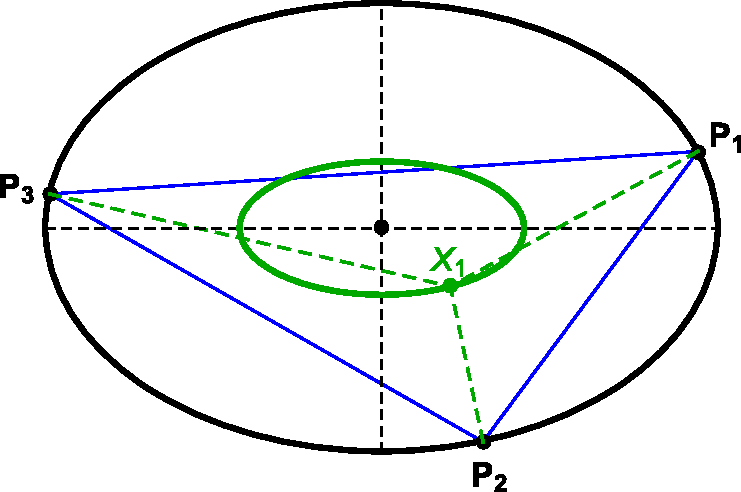
\includegraphics[height=.65\linewidth]{pics/0020_incenter_locus.pdf}
         \caption{The elliptic locus of the Incenter $X_1$.}
        \label{fig:locus-incenter}
     \end{subfigure}
     \hfill
     \begin{subfigure}[m]{0.45\textwidth}
         \centering
         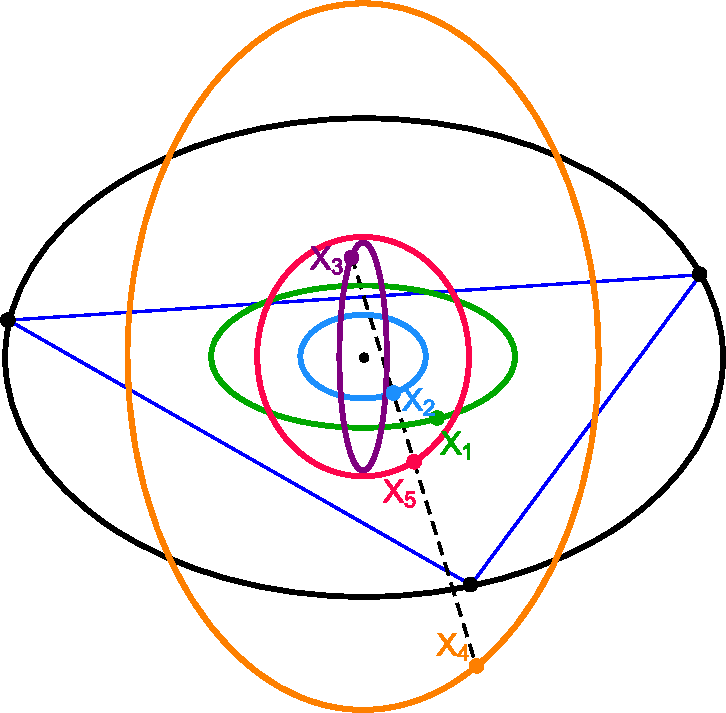
\includegraphics[height=\linewidth]{pics/0030_x12345_locus.pdf}
         \caption{Elliptic Loci of Incenter $X_1$, Barycenter $X_2$, Circumcenter $X_3$, Orthocenter $X_4$, and Center of the 9-Point Circle $X_5$.}
         \label{fig:locus-x12345}
     \end{subfigure}
     \caption{Elliptic Loci of major triangular centers.}
\end{figure}

\subsection{Eccentric Excenters}

Closely related to the Incenter are the {\em Excenters} \cite{mw}, the three meetpoints of perpendiculars to bisectors and vertices of the Excentral Triangle \cite{mw}. It turns out their locus is also elliptic and similar to a rotated version of the Incenter's  \cite{ronaldo19}, Figure~\ref{fig:locus-incenter-excenter}.
%

\begin{figure}[H]
    \centering
    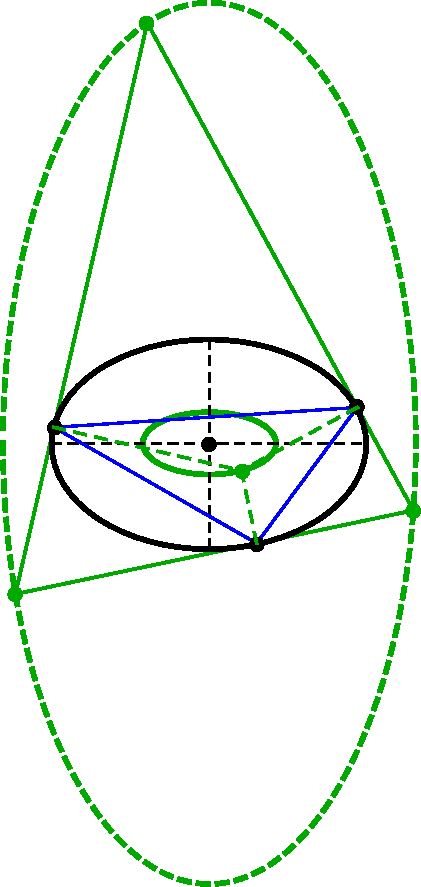
\includegraphics[angle=90,width=.73\textwidth]{pics/0025_incenter_excenter_locus.pdf}
    \caption{A Billiard is shown in black with its axes rotated (to save space), as well as an $N=3$ orbit (blue) and its Excentral Triangle (solid green). The vertices of the Excentral Triangle move along an elliptic locus similar to a perpendicular copy of the Incentral locus (shown solid green inside the Billiard).}
    \label{fig:locus-incenter-excenter}
\end{figure}

Though the vertices of the Excentral Triangle sweep an ellipse, consider those of the {\em Intouch Triangle}, formed by the three points of contact of the Incircle with the orbit. As shown in an early video \cite{dsr_vid11b}, their locus is self-intersecting with two lobes.

Generally, the locus of vertices of an orbit's derived triangle Figure~\ref{fig:derived-tris} are non-elliptic. Besides the Intouch vertices, those of the Feuerbach, and Medial Triangles \cite{mw} sweep non-elliptic curves. Surprisingly, the vertices of the {\em Extouch Triangle}, where Excircles touch the orbit sides, are not-only elliptic, but congruent with the Caustic! This is shown on Figure~\ref{fig:non-elliptic}.



\begin{figure}[H]
    \centering
    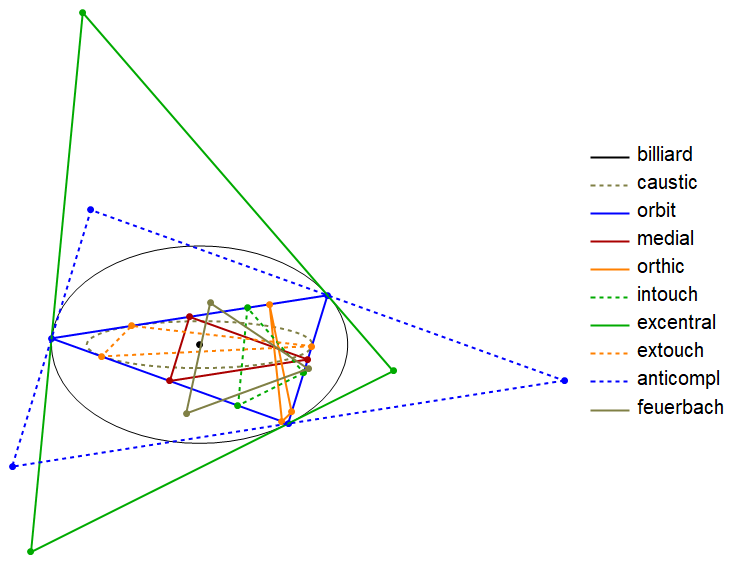
\includegraphics[width=.75\textwidth]{pics/0043_derived-triangles.png}
    \caption{A billiard is shown (black as well as an orbit (blue) and its Caustic (dashed brown). Several triangles derived from the orbit are shown, and indicated on the legend.}
    \label{fig:derived-tris}
\end{figure}
%
\begin{figure}[H]
    \centering
    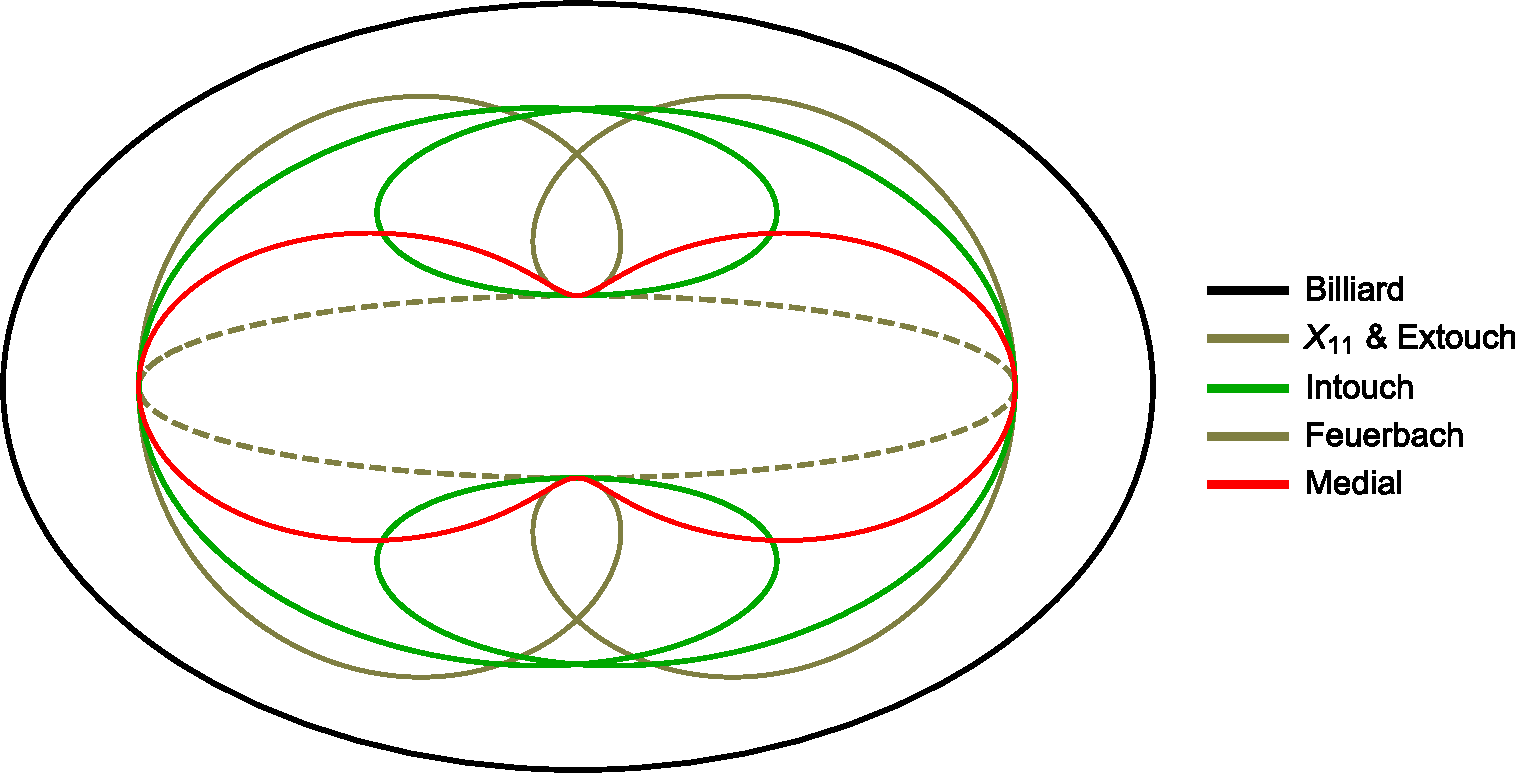
\includegraphics[height=.35\linewidth]{pics/0040_non_elliptic.pdf}
    \caption{The vertices of the Intouch (green), Feuerbach (brown), and Medial (red) Triangles sweep non-elliptic loci. Surprisingly, the extouch points (as well as the Feuerbach Point $X_{11}$, sweep the Caustic.}
    \label{fig:non-elliptic}
\end{figure}
The causes for ellipticity vs. non-ellipticity of loci of vertices of derived triangles is not   understood.
\subsection{Fiery Feuerbach}

The Feuerbach Point $X_{11}$ is the single point of contact between the Incircle and the 9-Point Circle \cite{mw}. Remarkably, and just like the vertices of the Extouch Triangle, its locus is also congruent with the $N=3$ Caustic Figure~\ref{fig:feuer_loci}.

Interestingly, if orbit vertices slide along the Billiard in one direction, $X_{11}$ (resp. the Extouch Points) will sweep the Caustic in the opposite (resp. same) direction \cite[video \#2]{dsr_main_videos_2019}.
%
\begin{figure}[H]
    \centering
    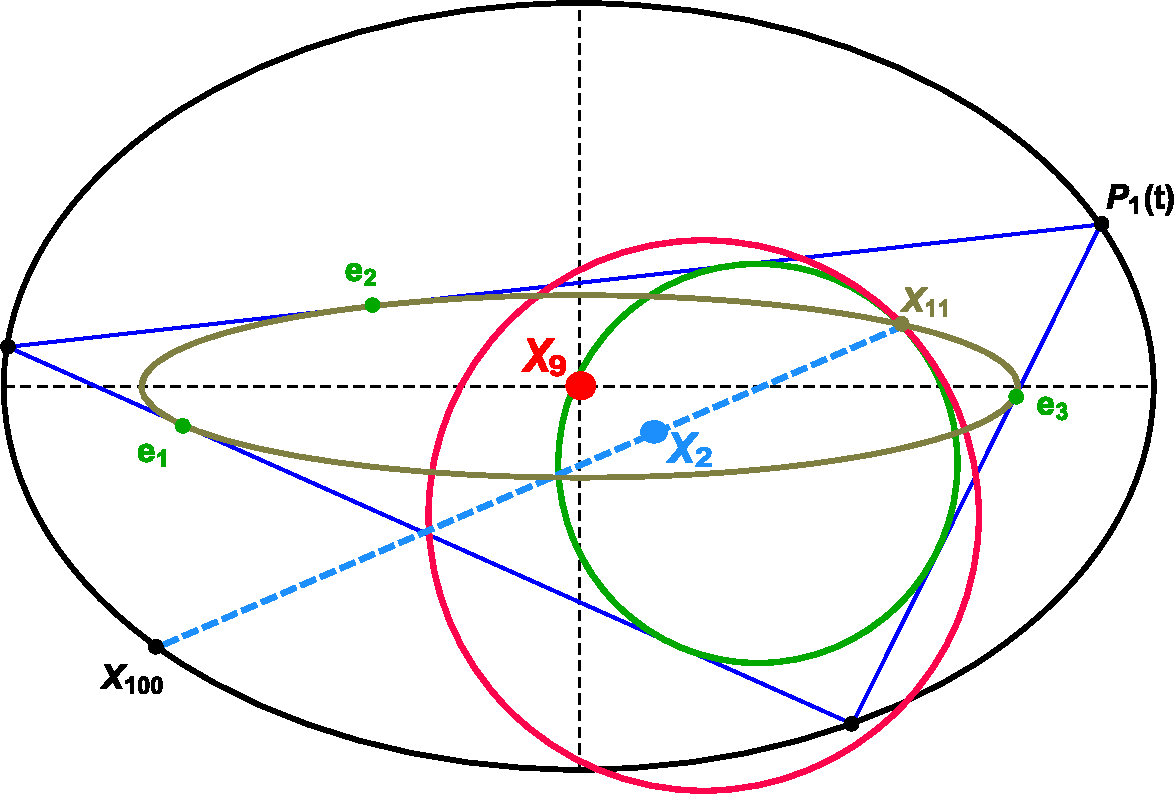
\includegraphics[width=.60\textwidth]{pics/0035_feuerbach_loci.pdf}
    \caption{Shown is the Elliptic Billiard (black), as well as an $N=3$ orbit (blue), with $P_1(t)$ the leader vertex, and the Caustic (brown). Also shown are the orbit's Incircle (green) and 9-Point Circle (pink), whose single point of contact is the Feuerbach Point $X_{11}$. Shown also is its anticomplement $X_{100}$, and the three Extouch Points $e_1,e_2,e_3$. Remarkable properties include: $X_{11}$ and the extouch points sweep the Caustic, and $X_{100}$ sweeps the Billiard (in opposite directions).}
    \label{fig:feuer_loci}
\end{figure}

Just as remarkably, $X_{100}$, the {\em anti-complement} \cite{mw} of the $X_{11}$, i.e., the latter's double-length reflection about the Barycenter $X_2$, is congruent with the Billiard \cite[video \#4]{dsr_main_videos_2019}. Also congruent with the Billiard, though not understood, is the locus of $X_{88}$.

\begin{observation}
The locus of $X_{11}$, the Feuerbach Point, is congruent with the $N=3$ Caustic and the locus of $X_{100}$, the anti-complement of the Feuerbach Point, is congruent with the Billiard, as is that of $X_{88}$.
\end{observation}

\subsection{First 100 Kimberling Points (only 39,900 more to go)}

Numerical analysis of the first 100 Kimberling Centers \cite{etc} reported that only 29 produce elliptic loci, listed on Table~\ref{tab:ell}. Also indicated is whether a given center centers are similar (or identical) to the Billiard, Caustic, or Excentral/Incentral Loci. The causes for the ellipticity (or non-ellipticity) of the locus of a Triangular Center haven't yet been uncovered.

\begin{table}[ht]
\caption{Ellipticity of Kimberling Centers}
\label{tab:ell}
$$
\begin{array}{cclcc}
\text{index} & \text{center} & \text{name} & \text{similarity} \\
\hline
 1 & X_{1}^* & \text{Incenter} & \text{J}^t \\
 2 & X_{2}^* & \text{Centroid} & \text{B} \\
 3 & X_{3}^* & \text{Circumcenter} & \text{C}^t  \\
 4 & X_{4}^* & \text{Orthocenter} & \text{B}^t \\
 5 & X_{5}^* & \text{9-Point Center} &  \\
 6 & X_{7}^* & \text{Gergonne Point} & \text{B}\\
 7 & X_{8}^* & \text{Nagel Point} &  \\
 8 & X_{10}^* & \text{Spieker Center} & \text{B}^t\\
 9 & X_{11}^* & \text{Feuerbach Point} & \text{C}^+ \\
 10 & X_{12}^* & \text{$\{X_{1},X_{5}\}$-Harmonic Conjugate of $X_{11}$} & \\
 11 & X_{20} & \text{de Longschamps Point} & \\
 12 & X_{21} & \text{Schiffler Point} & \\
 13 & X_{35} & \text{$\{X_{1},X_{3}\}$-Harmonic Conjugate of $X_{36}$} & \\
 14 & X_{36} & \text{Inverse-in-Circumcircle of Incenter} & \\
 15 & X_{40}^* & \text{Bevan Point} & \text{B}^t \\
 16 & X_{46} & \text{$X_{4}$-Ceva Conjugate of $X_{1}$} & \\
 17 & X_{55} & \text{Insimilicenter(Circumcircle,Incircle)} & \text{C}^+\\
 18 & X_{56} & \text{Exsimilicenter(Circumcircle,Incircle)} &  \\
 19 & X_{57}^* & \text{Isogonal Conjugate of $X_{9}$} &\text{B} \\
 20 & X_{63}^* & \text{Isogonal Conjugate of $X_{19}$} &\text{B} \\
 21 & X_{65}^* & \text{Orthocenter of the Intouch Triangle} & &\\
 22 & X_{72} & \text{Isogonal Conjugate of $X_{28}$} & \text{J}\\
 23 & X_{78} & \text{Isogonal Conjugate of $X_{34}$} & \\
 24 & X_{79} & \text{Isogonal Conjugate of $X_{35}$} & \\
 25 & X_{80} & \text{Reflection of Incenter in Feuerbach Point} &  \text{J}^t \\
 26 & X_{84} & \text{Isogonal Conjugate of $X_{40}$} & \\
 27 & X_{88}^* & \text{Isogonal Conjugate of $X_{44}$} &  \text{B}^+ \\
 28 & X_{90} & \text{$X_{3}$-Cross Conjugate of $X_{1}$} & \\
 29 & X_{100}^* & \text{Anticomplement of Feuerbach Point} & \text{B}^+\\
\end{array}
$$
\caption{The 29 Kimberling centers within $X_1$ to $X_{100}$ whose loci are elliptic. Entries under ``center'' which are starred entries identify centers whose locus has been {\em proven} as elliptic. Under ``similarity'', letters B,C,J indicate the locus is similar to Billiard, Caustic, or Excentral locus, respectively. An additional {+}  (resp. {t}) exponent indicates the locus is identical (resp. similar to a perpendicular copy) to the indicated ellipse.}
\end{table}

In Appendix~\ref{sec:locus-phenomena} we've placed further interesting locus phenomena such as (i) the quartic locus os the Symmedian $X_6$, so incredibly close to an ellipse, (ii) a locus with kinks (Incenter of the Orthic) and (iii) the Billiard-tracking locus of the contact points of the Anticomplementary Triangle. 